\documentclass[aps]{revtex4-1}

\usepackage{verbatim}
\usepackage{color}
\usepackage{epsfig}
\usepackage{float}
\usepackage{multirow}
\usepackage{amsfonts}
\usepackage{amssymb}
\usepackage{amsmath}
\usepackage{tabularx,url,color}
\usepackage{array}
\usepackage{hyperref}
\newcommand\bluenote[1]{\textcolor{blue}{\bf {#1}}}

\begin{document}
%\leftline{Dated: \today}

\title{Computer project at LAL: signal analysis of GW150914}

\begin{abstract}
  This paper describes the methods to analyze the data around GW150914 and to produce a multi-resolution spectrogram of the signal. The data time series is first whitened by the detector noise. Then the $Q$ transform is applied to perform a multi-resolution short Fourier transform of the data.
\end{abstract}

\author{
  Florent Robinet$^1$,  
}
        
\address{$^1$LAL, Univ. Paris-Sud, CNRS/IN2P3, Université Paris-Saclay, Orsay, France}

\maketitle

\tableofcontents

%%%%%%%%%%%%%%%%%%%%%%%%%%%%%%%%%%%%%%%%%%%%%%%%%%%%%%%%%%%%%%%%%
\section{The $Q$ transform} \label{sec:qtransform}
%%%%%%%%%%%%%%%%%%%%%%%%%%%%%%%%%%%%%%%%%%%%%%%%%%%%%%%%%%%%%%%%%
The data are processed using the $Q$ transform~\cite{Brown:1991}. The $Q$ transform is a modification of the standard short time Fourier transform in which the analysis window duration varies inversely with frequency such that the time-frequency plane is covered by tiles of constant quality factor $Q$. The signal time series, $x(t)$, is projected onto a basis of complex-valued windowed sine waves:
\begin{equation}
  X(\tau, \phi, Q) = \int_{-\infty}^{+\infty}{ x(t) w(t-\tau,\phi,Q) e^{-2i\pi\phi t}dt}.
  \label{eq:qtransform1}
\end{equation}
The transform coefficient, $X$, measures the average signal amplitude and phase within a time-frequency region, called a \textit{tile}, centered on time $\tau$ and frequency $\phi$, whose shape and area are determined by the requested quality factor $Q$ and the particular choice of analysis window, $w$. In~\cite{Gabor:1946}, it is shown that the minimal time-frequency resolution is achieved by a Gaussian window:
\begin{equation}
  w(t-\tau,\phi,Q) = \frac{W_g}{\sigma_t\sqrt{2\pi}}\exp\left [ -\frac{1}{2\sigma_t^2}(t-\tau)^2 \right],
  \label{eq:gausswindowt}
\end{equation}
where $W_g$ is a normalization factor and the Gaussian variance is $\sigma_t^2=\frac{Q^2}{8\pi^2\phi^2}$.

To optimize the algorithmic implementation of the $Q$ transform, we prefer an alternative form of Eq.~\ref{eq:qtransform1}, where we switch to the frequency domain using the Fourier transform defined as
\begin{equation}
  \tilde{x}(f) = \int_{-\infty}^{+\infty}{ x(t) e^{-2i\pi f t}dt}. \label{eq:FTforward}
\end{equation}
The corresponding reverse Fourier transform is
\begin{equation}
  x(t) = \int_{-\infty}^{+\infty}{ \tilde{x}(f) e^{2i\pi f t}df}.  \label{eq:FTbackward}
\end{equation}
Using the inverse Fourier transform, the cross-correlation theorem, the Fourier transform translation relation and the fact that we are working with a real window, we can re-write Eq~\ref{eq:qtransform1}:
\begin{align}
  X(\tau, \phi, Q) &= \int_{-\infty}^{+\infty}{\tilde{X}(f,\phi,Q) e^{+2i\pi f \tau}df} \\
  X(\tau, \phi, Q) &= \int_{-\infty}^{+\infty}{ \widetilde{\left (\int_{-\infty}^{+\infty}{w^*(t,\phi,Q)x(t+\tau)e^{-2i\pi\phi(t+\tau)}dt}\right)} e^{+2i\pi f \tau}df}\\
  X(\tau, \phi, Q) &= \int_{-\infty}^{+\infty}{ \tilde{x}(f+\phi) \tilde{w}^{*}(f,\phi,Q) e^{+2i\pi f \tau}df}.
  \label{eq:qtransform2}
\end{align}
In Eq.~\ref{eq:qtransform2}, the signal is applied a Fourier transform, a shift in frequency, a multiplication by the frequency-domain window and an inverse Fourier transform.

%%%%%%%%%%%%%%%%%%%%%%%%%%%%%%%%%%%%%%%%%%%%%%%%%%%%%%%%%%%%%%%%%
\section{The window} \label{sec:window}
%%%%%%%%%%%%%%%%%%%%%%%%%%%%%%%%%%%%%%%%%%%%%%%%%%%%%%%%%%%%%%%%%
To compute the $Q$ transform of Eq.~\ref{eq:qtransform2}, we need to apply a Fourier transform to the Gaussian window of Eq.~\ref{eq:gausswindowt}. In the frequency domain, the window is also Gaussian and real:
\begin{equation}
  \tilde{w}(f,\phi,Q) = \tilde{w}^*(f,\phi,Q) = W_g\exp\left [ -\frac{1}{2\sigma_f^2}f^2 \right],
  \label{eq:gausswindowf}
\end{equation}
where $\sigma_f^2=\frac{2\phi^2}{Q^2}$.

The Gaussian window provides the best time-frequency resolution~\cite{Gabor:1946}. However, such a window has an infinite extent which makes it difficult to use in a discrete analysis framework. Instead, we approximate the Gaussian window with a bisquare window which has a simple form in the frequency domain:
\begin{equation}
  \tilde{w}(f,\phi,Q) = \tilde{w}^*(f,\phi,Q) =
  \begin{cases}
    W_b\left[1 - \left(\frac{f}{\delta_f(\phi,Q)}\right)^2 \right]^2 & |f| < \delta_f(\phi,Q), \\
    0 & \textrm{otherwise},
  \end{cases}
  \label{eq:bisquare}
\end{equation}
where $W_b$ is a normalization factor and $\delta_f(\phi,Q)=\phi\sqrt{11}/Q$ is the half size of the window.

Thanks to the finite extent of the the bisquare window, it is possible to add protections against signal aliasing. Indeed, when using the two conditions
\begin{align}
  &Q\ge\sqrt{11} \qquad \text{and}\label{eq:antialias1} \\
  &\phi \le \frac{f_{\text{Nyquist}}}{1+\sqrt{11}/Q}, \label{eq:antialias2}
\end{align}
the zero frequency and the Nyquist frequency, $f_{\text{Nyquist}}$, are never exceeded: $0 \le f + \phi \le f_{\text{Nyquist}}$. The $Q$ transform in Eq.~\ref{eq:qtransform2} can, therefore, be safely discretized.

The window normalization factor is such that
\begin{equation}
  \int_{-\infty}^{+\infty}{|\tilde{w}(f,\phi,Q)|^2df} = 2.
  \label{eq:winnorm}
\end{equation}
Using this normalization condition has many advantages. A trivial integration yields the normalization factor for the bisquare window
\begin{equation}
  W_b = \sqrt{\frac{315}{128\sqrt{11}} \frac{Q}{\phi}},
  \label{eq:Wb}
\end{equation}
while for the Gaussian case we get
\begin{equation}
  W_g = \sqrt{\frac{2}{\sqrt{\pi}\sigma_f}} = \sqrt{\sqrt{\frac{2}{\pi}} \frac{Q}{\phi}},
  \label{eq:Wg}
\end{equation}

A characteristic duration, $\Delta t$, and bandwidth, $\Delta f$, are defined using the second central moments of the window:
\begin{align}
  \left(\frac{\Delta f}{2}\right)^2 &= \int_{-\infty}^{+\infty}{f^2|\tilde{w}(f,\phi,Q)|^2 df}\\
  \left(\frac{\Delta t}{2}\right)^2 &= \int_{-\infty}^{+\infty}{t^2|w(t,\phi,Q)|^2 dt}.
\end{align}
For both the Gaussian and bisquare windows, we naturally find indentical values:
\begin{align}
  \Delta f &=  2\sigma_f = 2\sqrt{2}\frac{\phi}{Q},  \label{eq:sigf} \\ 
  \Delta t &=  2\sigma_t = \frac{1}{\sqrt{2}\pi}\frac{Q}{\phi}. \label{eq:sigt}
\end{align}

In the following, we will often refer to a basis of complex-valued sinusoidal Gaussian waveforms keeping in mind that bisquare windows are actually used.

%%%%%%%%%%%%%%%%%%%%%%%%%%%%%%%%%%%%%%%%%%%%%%%%%%%%%%%%%%%%%%%%%
\section{The tiles} \label{sec:tiles}
%%%%%%%%%%%%%%%%%%%%%%%%%%%%%%%%%%%%%%%%%%%%%%%%%%%%%%%%%%%%%%%%%
The tiles must be chosen to cover a finite region of parameter space, $[\tau_{min};\tau_{max}]\times [\phi_{min};\phi_{max}] \times [Q_{min};Q_{max}]$. The density of tiles must be large to guarantee a high detection efficiency. However, the number of tiles must also be as small as possible to provide a fast processing. To meet these two competitive requirements, the parameter space is tiled such that the fractional energy loss due to mismatch is below a pre-defined value, $\mu_{max}$. For complex-valued sinusoidal Gaussian waveforms, the mismatch can be analytically computed and the optimal number of tiles can be determined. The tiles are distributed over a cubic lattice using a mismatch metric~\footnote{The metric includes a non-diagonal $\delta \phi \delta Q$ term which has been neglected.} to measure distances:
\begin{equation}
  \delta s^2 =
  \frac{4\pi^2\phi^2}{Q^2}\delta \tau^2
  + \frac{2+Q^2}{4\phi^2}\delta \phi^2
  + \frac{1}{2Q^2}\delta Q^2.
  \label{eq:tilemetric}
\end{equation}
To guarantee a fractional energy loss smaller than $\mu_{max}$, the minimum number of tiles, $N_\tau \times N_\phi \times N_Q$, is given by the mismatch distances integrated over the three dimensions:
\begin{align}
  N_\tau \ge \frac{s_\tau}{2\sqrt{\mu_{max}/3}},  & \qquad s_\tau = \frac{2\pi\phi}{Q}(\tau_{max} - \tau_{min}), \label{eq:tiledistancetau} \\
  N_\phi \ge \frac{s_\phi}{2\sqrt{\mu_{max}/3}},  & \qquad s_\phi = \frac{\sqrt{2+Q^2}}{2}\ln(\phi_{max}/\phi_{min}), \label{eq:tiledistancephi} \\
  N_Q \ge \frac{s_Q}{2\sqrt{\mu_{max}/3}},  & \qquad s_Q = \frac{1}{\sqrt{2}}\ln(Q_{max}/Q_{min}). \label{eq:tiledistanceq}
\end{align}
This tiling structure can be depicted as a set of $N_Q$ logarithmically-spaced $Q$ planes, indexed by $q$:
\begin{equation}
  Q_q = Q_{min}\left[ \frac{Q_{max}}{Q_{min}}\right]^{(0.5+q)/N_q}, \qquad 0\le q < N_Q.
  \label{eq:q}
\end{equation}
Each of these planes is divided into $N_\phi(Q_q)$ logarithmically-spaced frequency rows, indexed by $q$ and $l$:
\begin{equation}
  \phi_{ql} = \phi_{min}\left[ \frac{\phi_{max}}{\phi_{min}}\right]^{(0.5+l)/N_\phi(Q_q)}, \qquad 0\le l < N_\phi(Q_q).
  \label{eq:phi}
\end{equation}
Each frequency row is finally sub-divided into $N_\tau(Q_q,\phi_{ql})$ linearly-spaced time bins, indexed by $q$, $l$ and $m$:
\begin{equation}
  \tau_{qlm} = \tau_{min}+(m+0.5)\frac{\tau_{max}-\tau_{min}}{N_\tau(Q_q,\phi_{ql})}, \qquad 0\le m < N_\tau(Q_q,\phi_{ql}).
  \label{eq:tau}
\end{equation}

The targeted parameter space must be specified: the $Q$ range, $[Q_{min}; Q_{max}]$, the frequency range, $[\phi_{min}; \phi_{max}]$ and a time range. The time range is fixed to the characteristic chunk duration, $T_c$, and is centered on 0: $[-T_c/2; +T_c/2]$. If necessary, the $Q_{min}$ and $\phi_{max}$ parameters are automatically adjusted so that they verify the anti-aliasing conditions of Eq.~\ref{eq:antialias1} and Eq.~\ref{eq:antialias2}. In addition, it is required to work with an integrated mismatch distance along the time dimension $s_\tau\ge4$, which translates into a minimum permissible frequency, $\phi_{min} \ge 2Q/(\pi T_c)$.

A $Q$ plane object is implemented as a C++ class inheriting from the 2-D histogram class of ROOT (\texttt{TH2D}). The number of $Q$ planes, $N_Q$, is equal to the next integer verifying condition of Eq.~\ref{eq:tiledistanceq}. The $Q$ planes, indexed by $q$, are given a $Q$ value obtained from Eq.~\ref{eq:q}.

A $Q$ plane histogram is then vertically binned into logarithmically-spaced frequency rows. The number of frequency rows, $N_\phi(Q_q)$, is equal to the next integer verifying condition of Eq.~\ref{eq:tiledistancephi}. For each frequency row $(q,l)$, the horizontal time axis is divided into $N_\tau(Q_q,\phi_{ql})$ linear bins, $N_\tau(Q_q,\phi_{ql})$ being the next power of two verifying the condition of Eq.~\ref{eq:tiledistancetau}. Indeed, in Sec.~\ref{sec:discrete}, we explain that working with power-of-two vector sizes is computationally more efficient when performing Fourier transforms. The tile time and frequency, $(\tau_{qlm}, \phi_{ql})$, is given by the histogram bin center obtained from~Eq.\ref{eq:tau} and Eq.~\ref{eq:phi}. It is also useful to give the histogram bin width in both the time and frequency dimensions:
\begin{align}
  \Delta\tau_{ql} &= T_c / N_\tau(Q_q, \phi_{ql}), \label{eq:dtau} \\
  \Delta\phi_{ql} &= 4\phi_{ql}\sqrt{\frac{\mu_{max}}{3(2+Q_q^2)}}.\label{eq:dphi}
\end{align}

A realistic example of a tiling structure is represented in Fig.~\ref{fig:tiling}.
\begin{figure}
  \center
  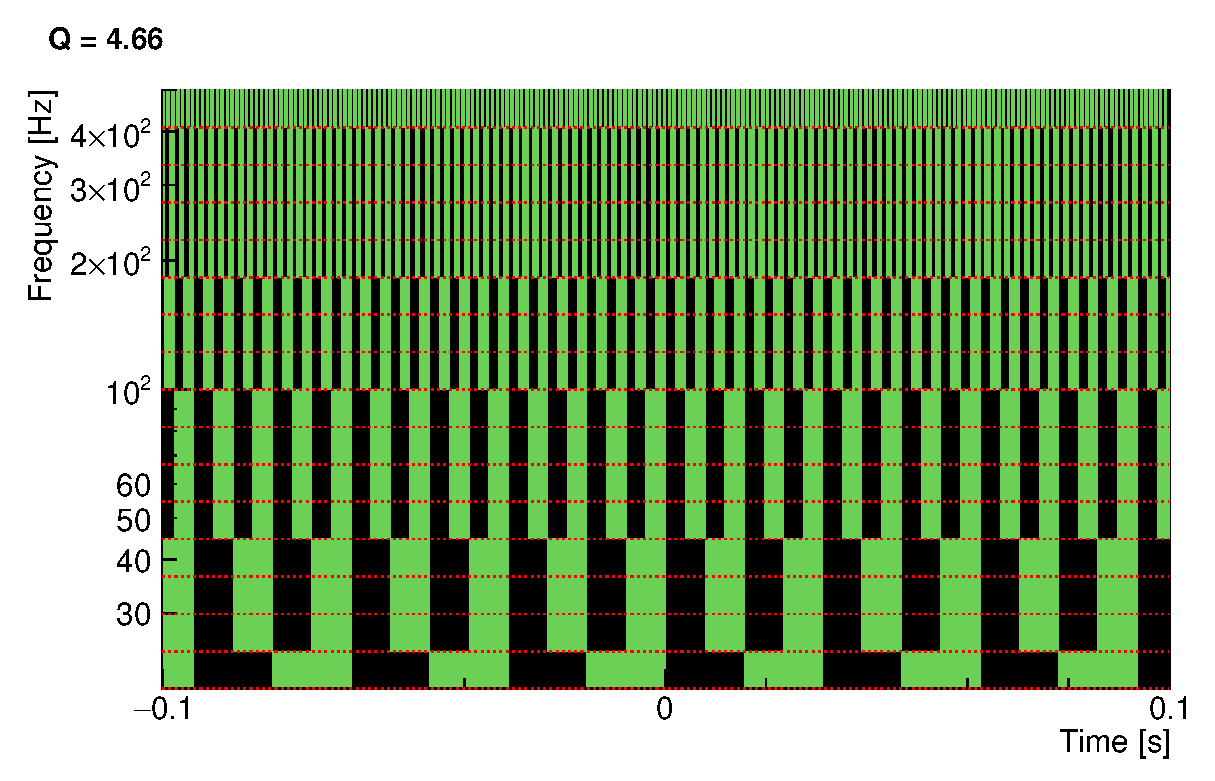
\epsfig{width=7.5cm, file=./q0.eps} 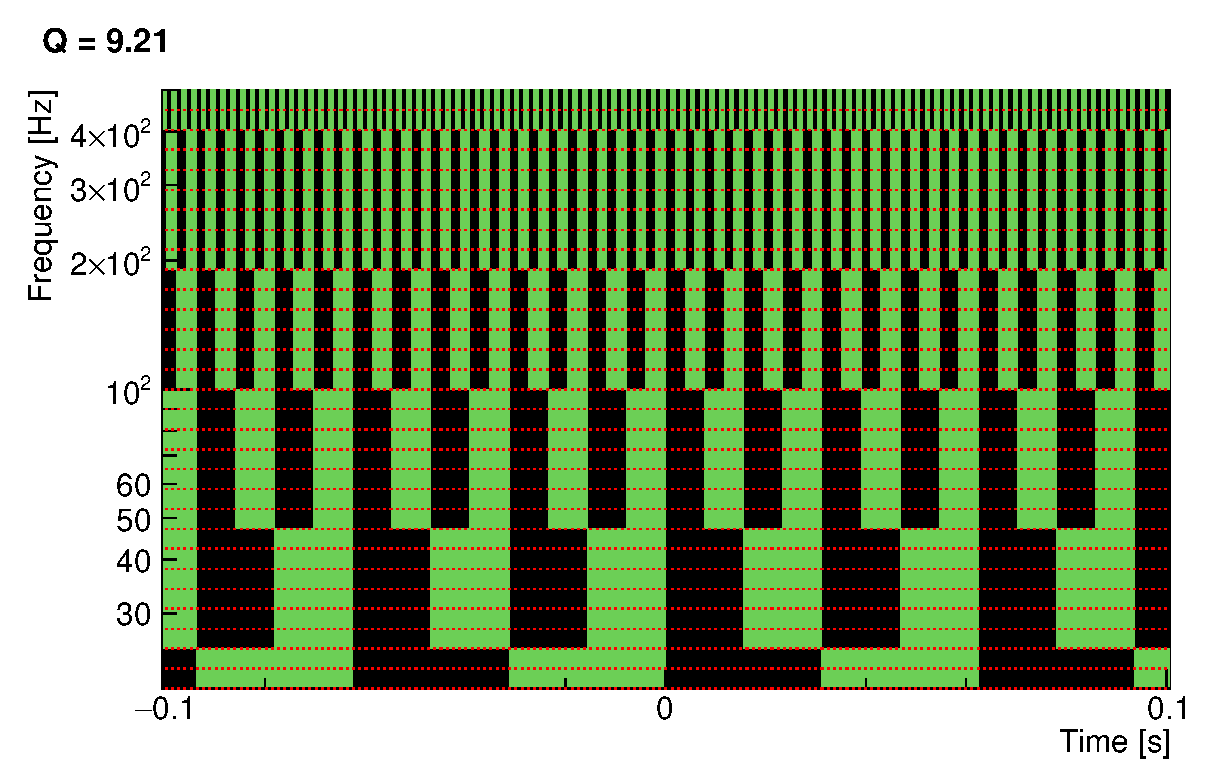
\epsfig{width=7.5cm, file=./q1.eps} \\
  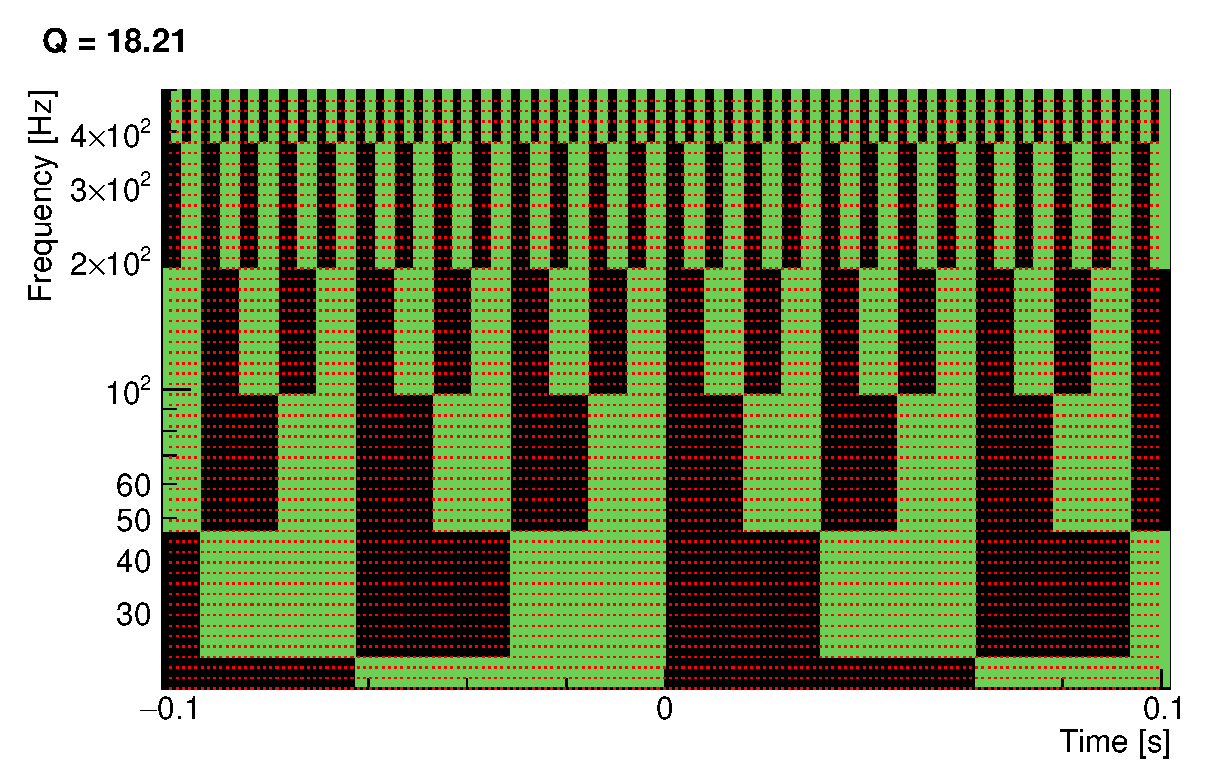
\epsfig{width=7.5cm, file=./q2.eps} 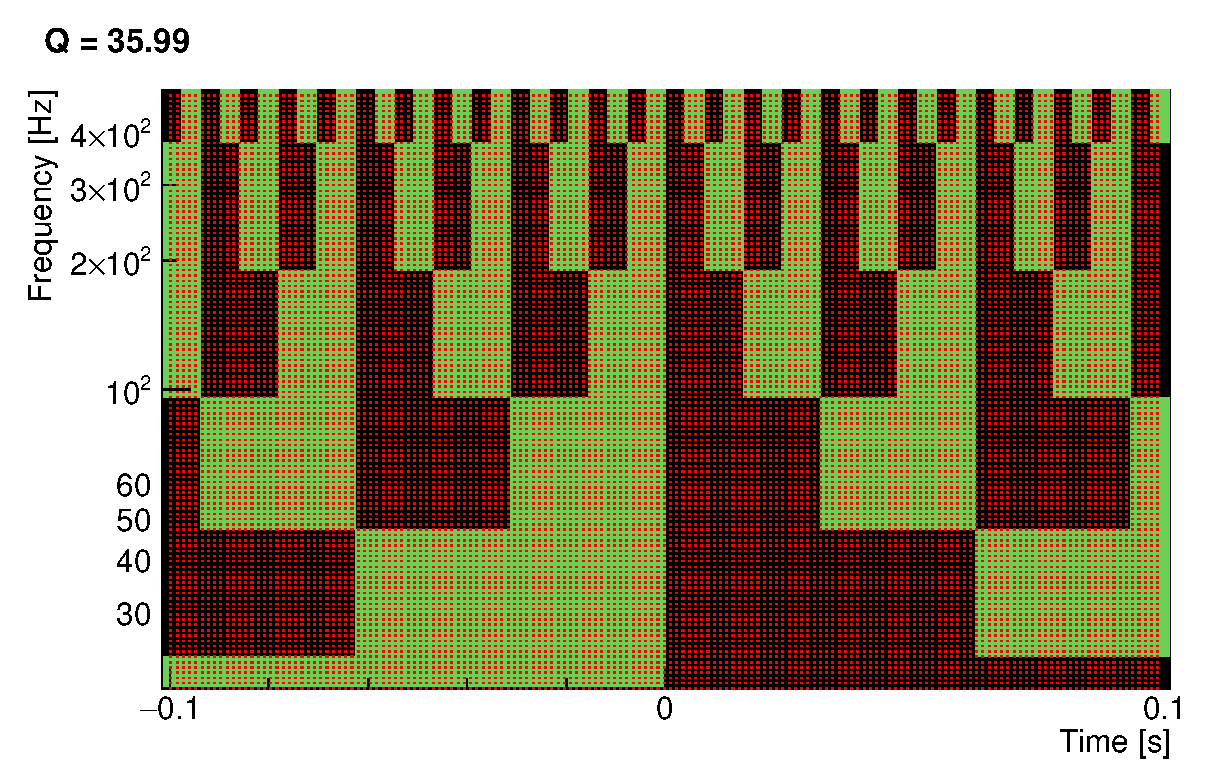
\epsfig{width=7.5cm, file=./q3.eps} \\
  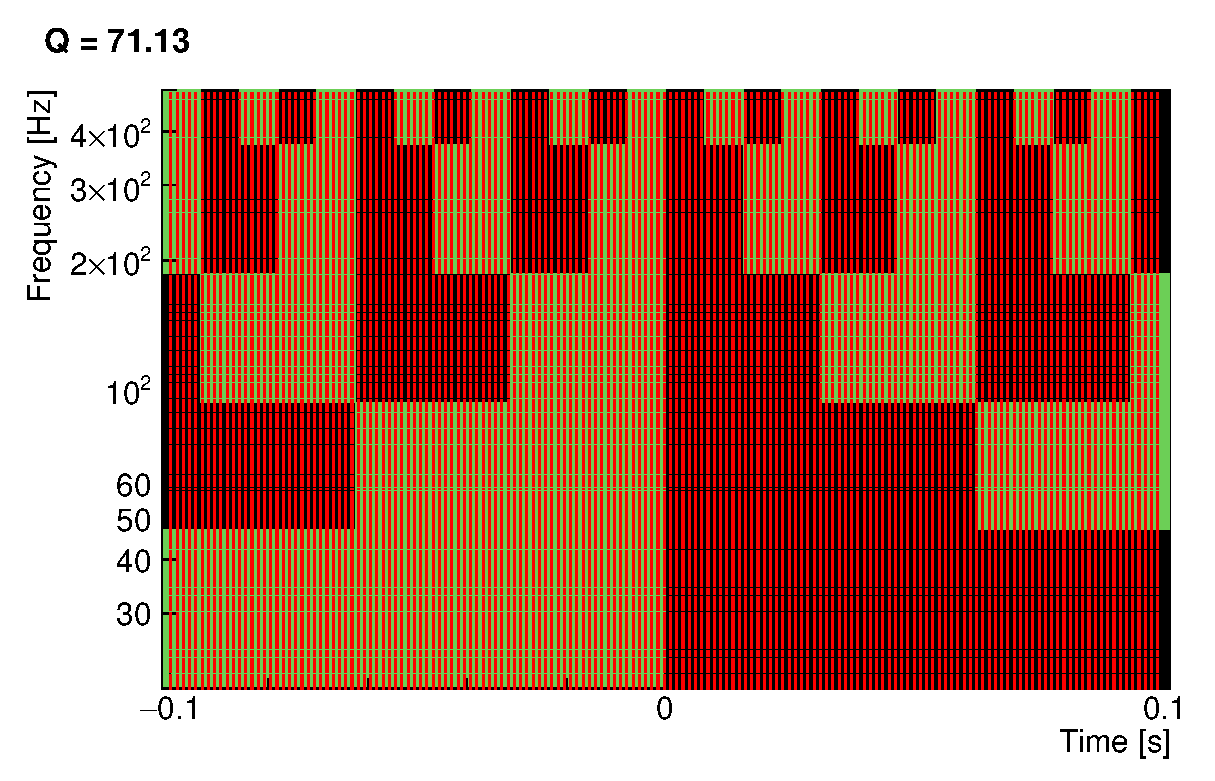
\epsfig{width=7.5cm, file=./q4.eps}
  \caption{Example of a realistic tiling structure. When requiring a maximal energy loss of $\mu_{max}=20\%$, 5 $Q$ planes are needed to cover the $Q$ range $[\sqrt{11}; 100]$. Each $Q$ plane is then tiled (black and green rectangles) along frequency rows delimited by the red dashed lines. To distinguish the tiles, the time chunk is zoomed in $\pm 100$~ms.}
  \label{fig:tiling}
\end{figure}

%%%%%%%%%%%%%%%%%%%%%%%%%%%%%%%%%%%%%%%%%%%%%%%%%%%%%%%%%%%%%%%%%
\section{The noise whitening} \label{sec:whitening}
%%%%%%%%%%%%%%%%%%%%%%%%%%%%%%%%%%%%%%%%%%%%%%%%%%%%%%%%%%%%%%%%%
Whitening the noise before applying the $Q$ transform is useful for a subsequent statistical interpretation of the $Q$ transform coefficients. To achieve this, a simple method consists of re-weighting the frequency-domain data by the inverse noise amplitude spectral density:
\begin{equation}
  \tilde{x}^{wh}(f) = \frac{\tilde{x}(f)}{\sqrt{S_n(|f|)/2}},
  \label{eq:whitening}
\end{equation}
where $S_n(f)$ is the one-sided ($f \ge 0$) noise power spectrum density (PSD). After this transformation, the power of a random noise process is equally distributed over the frequencies and the one-sided PSD of $x^{wh}$ is flat and equal to 2.

The noise one-sided PSD is usually estimated by averaging multiple one-sided periodograms computed over a finite duration $T$ (Welch method):
\begin{equation}
  P_T(f) = \frac{2}{T}\left|\tilde{x}_T(f)\right|^2, \qquad f \ge 0.
  \label{eq:periodogram}
\end{equation}
In a one-sided convention, the factor 2 accounts for the negative frequencies of $\tilde{x}_T$. Note that this factor is corrected back when whitening the data in Eq.~\ref{eq:whitening}.

%%%%%%%%%%%%%%%%%%%%%%%%%%%%%%%%%%%%%%%%%%%%%%%%%%%%%%%%%%%%%%%%%
\section{The signal-to-noise ratio} \label{sec:snr}
%%%%%%%%%%%%%%%%%%%%%%%%%%%%%%%%%%%%%%%%%%%%%%%%%%%%%%%%%%%%%%%%%
Let's consider a burst of energy, the waveform of which is $b(t)$. It lies on top of noise, $n(t)$, such as $x(t) = b(t) + n(t)$. An amplitude $Q$ transform signal-to-noise ratio (SNR) for each tile is defined as
\begin{equation}
  \rho_{qlm}^2 =  \frac{|X_b(\tau_{qlm}, \phi_{ql}, Q_q)|^2}{\langle |X_n(\tau_{qlm}, \phi_{ql}, Q_q)|^2 \rangle/2}, \label{eq:snrdef}
\end{equation}
where $X_b(\tau_{qlm}, \phi_{ql}, Q_q)$ is the $Q$ transform coefficient for the burst waveform in tile $(q,l,m)$. The expectation value of the $Q$ transform energies for noise in tile $(q,l,m)$, obtained from multiple measurements, is given by $\langle |X_n(\tau_{qlm}, \phi_{ql}, Q_q)|^2\rangle$.

The SNR definition given by Eq.~\ref{eq:snrdef} is consistent with the maximum achievable SNR defined in the framework of the matched filter theory~\cite{helstrom:1968}. To demonstrate this, let's consider a burst test signal exactly matching the tile under consideration. The burst waveform is a sinusoidal Gaussian function of time, the parameters of which match the tile $(q,l,m)$:
\begin{align}
  b(t) &= Bw(t-\tau_{qlm}, \phi_{ql}, Q_q)\cos(2\pi\phi_{ql} t + \theta_{bt}), \label{eq:sg_wave}\\
  \tilde{b}(f) &= \frac{B}{2}e^{-2i\pi f\tau_{qlm}}\left[ \tilde{w}(f-\phi_{ql},\phi_{ql},Q_q)e^{-2i\pi\tau_{qlm}(f-\phi_{ql})}e^{i\theta_{bt}}+\tilde{w}(f+\phi_{ql},\phi_{ql},Q_q)e^{-2i\pi\tau_{qlm}(f+\phi_{ql})}e^{-i\theta_{bt}}\right],
\end{align}
where $B$ is the signal amplitude and $\theta_{bt}$ is the arbitrary phase between the burst and the tile. Using the frequency-domain $Q$ transform of Eq.~\ref{eq:qtransform2}, we compute the squared magnitude of the $Q$ transform coefficient, or energy, for tile $(q,l,m)$:
\begin{align}
  |X_b(\tau_{qlm}, \phi_{ql}, Q_q)|^2 &= \left|\int_{-\infty}^{+\infty}{ \frac{B}{2}\left[ \tilde{w}(f,\phi_{ql},Q_q)+\tilde{w}(f+2\phi_{ql},\phi_{ql},Q_q)\right] \tilde{w}^{*}(f,\phi_{ql},Q_q) df} \right|^2\\
  &= \left|\int_{-\infty}^{+\infty}{ \frac{B}{2} \tilde{w}(f,\phi_{ql},Q_q) \tilde{w}^{*}(f,\phi_{ql},Q_q) df}\right|^2 \\
  &= B^2,
  \label{eq:qtransform_signal}
\end{align}
where we used the window normalization of~Eq.\ref{eq:winnorm} and the fact that $\tilde{w}^{*}(f,\phi_b,Q_b)\tilde{w}(f+2\phi_b,\phi_b,Q_b)=0$ if we use the bisquare window approximation verifying condition of Eq.~\ref{eq:antialias1}.

Now, let's estimate the mean squared magnitude of the $Q$ transform coefficient for the noise in the denominator of Eq.~\ref{eq:snrdef}. We assume that the noise, $n(t)$, is a stationary stochastic process. With this assumption, the expectation value $\langle |X_n(\tau_{qlm}, \phi_{ql}, Q_q)|^2 \rangle$ is time-independent and the $\tau$ dependency can be dropped:
\begin{equation}
  \langle |X_n(\tau_{qlm}, \phi_{ql}, Q_q)|^2 \rangle = \langle |X_n(\phi_{ql}, Q_q)|^2 \rangle = \int_{-\infty}^{+\infty}{ \int_{-\infty}^{+\infty}{ \langle n(t)n^*(t') \rangle w(t,\phi_{ql},Q_q) w^*(t',\phi_{ql},Q_q) e^{-2i\pi\phi_{ql}(t-t')}dt}dt'}.
  \label{eq:qtransform_noise1}
\end{equation}
Then we can use the Wiener-Khinchin theorem, defining the one-sided power spectrum density of a stationary noise process,
\begin{equation}
  S_n(f)=2\int_{-\infty}^{+\infty}{ \langle n(t)n^*(t-T) \rangle e^{-2i\pi fT}dT},\qquad f\ge0
\end{equation}
and the autocorrelation theorem,
\begin{equation}
  \int_{-\infty}^{+\infty}{w(t)w^*(t-T)dt} = \int_{-\infty}^{+\infty}{|\tilde{w}(f)|^2e^{2i\pi fT}df},
\end{equation}
to re-write Eq.~\ref{eq:qtransform_noise1}:
\begin{equation}
  \langle |X_n(\tau_{qlm}, \phi_{ql}, Q_q)|^2 \rangle =  \frac{1}{2}\int_{-\infty}^{+\infty}{ |\tilde{w}(\phi_{ql}-f,\phi_{ql},Q_q)|^2S_n(|f|) df }.
  \label{eq:qtransform_noise}
\end{equation}
Taking into account the normalization condition of Eq.~\ref{eq:winnorm}, the mean squared magnitude of the $Q$ transform coefficient for a stationary stochastic process can be interpreted as the noise power density integrated over the tile frequency window. Moreover, if we consider that the power spectral density is approximately constant over the window bandwidth, we get $\langle |X_n(\tau_{qlm}, \phi_{ql}, Q_q)|^2 \rangle \simeq S_n(\phi_{ql})$. This result, combined with Eq.~\ref{eq:qtransform_signal}, can be used to derive the SNR defined by Eq.~\ref{eq:snrdef}:
\begin{equation}
  \rho_{qlm} \simeq  \frac{B}{\sqrt{S_n(\phi_{ql})/2}}.
  \label{eq:snrmatch}
\end{equation}
As previously announced, this result is exactly what is obtained in the context of the matched filtering theory~\cite{helstrom:1968}. The factor 2 is used to correct for the power of negative frequencies folded in the one-sided PSD.

One must recall that the $Q$ transform is performed after whitening the time series as described in Sec.~\ref{sec:whitening}. The above calculation must therefore be modified. In particular, Eq.~\ref{eq:qtransform_signal} and Eq.~\ref{eq:qtransform_noise} become:
\begin{align}
  |X^{wh}_b(\tau_{qlm}, \phi_{ql}, Q_q)| &= B \int_{-\infty}^{+\infty}{\frac{|\tilde{w}(f-\phi_{ql},\phi_{ql},Q_q)|^2}{2\sqrt{S_n(|f|)/2}}df}, \\
  \langle |X^{wh}_n(\tau_{qlm}, \phi_{ql}, Q_q)|^2 \rangle &= 2.
  \label{eq:qtransform_whitened}
\end{align}
The SNR is then given by
\begin{equation}
  \rho_{qlm} = |X^{wh}_b(\tau_{qlm}, \phi_{ql}, Q_q)| = B \int_{-\infty}^{+\infty}{\frac{|\tilde{w}(f-\phi_{ql},\phi_{ql},Q_q)|^2}{2\sqrt{S_n(|f|)/2}}df},
  \label{eq:snr_white}
\end{equation}
and the special case of Eq.~\ref{eq:snrmatch} remains true.

~

For obvious reasons, the burst signal cannot be disentangled from noise; only $x$ is measured. As a result, the SNR of Eq.~\ref{eq:snrdef} cannot be exactly computed. Instead, it is estimated using the $Q$ transform coefficient of $x$:
\begin{equation}
  \hat{\rho}_{qlm}^2 =  |X^{wh}(\tau_{qlm}, \phi_{ql}, Q_q)|^2 - \langle |X^{wh}_n(\tau_{qlm}, \phi_{ql}, Q_q)|^2 \rangle .
\end{equation}
As mentioned above, the $Q$ transform expectation value for a white noise is 2. Therefore the SNR estimator takes the simple form
%However we prefer to keep a general expression because, as we will see in Sec.~\ref{sec:algorithm:snr}, the whitening procedure is not perfect. As a result, the noise expectation value $\langle |X^{wh}_n(\tau_{qlm}, \phi_{ql}, Q_q)|^2 \rangle$ must be estimated.
\begin{equation}
  \hat{\rho}_{qlm}^2 =  |X^{wh}(\tau_{qlm}, \phi_{ql}, Q_q)|^2 - 2 . \label{eq:snrestimator}
\end{equation}

Now, let's estimate how correct our SNR estimator is. The squared magnitude of the $Q$ transform coefficient of $x=b+n$ for tile $(q,l,m)$ can be expanded as
\begin{equation}
  |X(\tau_{qlm}, \phi_{ql}, Q_q)|^2 = |X_b(\tau_{qlm}, \phi_{ql}, Q_q)|^2 + |X_n(\tau_{qlm}, \phi_{ql}, Q_q)|^2 + 2|X_n(\tau_{qlm}, \phi_{ql}, Q_q)|\ |X_b(\tau_{qlm}, \phi_{ql}, Q_q)|\cos{\theta_{bn}},
\end{equation}
where $\theta_{bn}$ is the phase between the burst and the noise signals. Using this expression, and switching to whitened quantities, the SNR estimator can be re-written as
\begin{equation}
  \hat{\rho}_{qlm}^2  =
  \rho_{qlm}^2
%  + |X^{wh}_n(\tau_{qlm}, \phi_{ql}, Q_q)|^2 - \langle |X^{wh}_n(\tau_{qlm}, \phi_{ql}, Q_q)|^2 \rangle
  + |X^{wh}_n(\tau_{qlm}, \phi_{ql}, Q_q)|^2 - 2
  + 2|X^{wh}_n(\tau_{qlm}, \phi_{ql}, Q_q)|\ |X^{wh}_b(\tau_{qlm}, \phi_{ql}, Q_q)| \cos{\theta_{bn}}.
  \label{eq:snrbias}
\end{equation}
From this expression, we see that our SNR estimate can differ from the true value because of two causes: the random fluctuations of white noise around the mean value and the arbitrary phase, $\theta_{bn}$, between the burst and the noise signals. For both cases, distributions are known. In~\cite{Chatterji:2004}, it is shown that the distribution of $|X^{wh}_n(\tau_{qlm}, \phi_{ql}, Q_q)|^2$ is exponential with mean $\langle |X^{wh}_n(\tau_{qlm}, \phi_{ql}, Q_q)|^2 \rangle = 2$. The standard deviation of $|X^{wh}_n(\tau_{qlm}, \phi_{ql}, Q_q)|^2$ from 2 is therefore 2. In addition, assuming that the signal and the noise are independent, the distribution of the phase $\theta_{bn}$ is uniform over all angles.

%%%%%%%%%%%%%%%%%%%%%%%%%%%%%%%%%%%%%%%%%%%%%%%%%%%%%%%%%%%%%%%%%
\section{The discrete analysis} \label{sec:discrete}
%%%%%%%%%%%%%%%%%%%%%%%%%%%%%%%%%%%%%%%%%%%%%%%%%%%%%%%%%%%%%%%%%

The data consists of a discrete time sequence, $x[j]$, which is identified by a channel name and a native sampling frequency, $f_s$, defining the time separation between two consecutive data points $\delta t = t_{j+1}-t_j = 1/f_s$. The forward and inverse Fourier transforms of Eq.~\ref{eq:FTforward} and~\ref{eq:FTbackward} are discretized as 
\begin{equation}
  \tilde{x}[k]=\frac{1}{f_s}\sum_{j=0}^{N-1}{x[j]\mathrm{e}^{-2i\pi jk/N}}
  \label{eq:dFTforward}
\end{equation}
and
\begin{equation}
  x[j]=\frac{f_s}{N}\sum_{k=0}^{N-1}{\tilde{x}[k]\mathrm{e}^{+2i\pi jk/N}}.
  \label{eq:dFTbackward}
\end{equation}
The frequency-domain data vector, $\tilde{x}$, is of size $N$ and the frequency sample interval is $\delta f = f_{k+1}-f_k = f_s/N = 1/T$. By convention, the first element, $\tilde{x}[0]$ is the DC component which is a purely real number. Positive frequencies are stored in the first half of $\tilde{x}$: $f_k=kf_s/N$, with $1\le k \le N/2$. The element $\tilde{x}[N/2]$ is purely real and is associated to the Nyquist frequency $f_{\text{Nyquist}}=f_s/2$. Negative frequencies are stored backward in the second half of $\tilde{x}$: $f_k=(k-N)f_s/N$, with $N/2 < k < N$.

Discrete Fourier transforms are performed with the FFTW~\cite{FFTW} algorithm. They can be computationally expensive and care must be taken to optimize the use of FFTW routines. A first approach is to only work with vector sizes which are a power of two. With such a configuration, the FFTW routines provide optimal performance. Another possibility of optimization is to take advantage from the fact that, most often, we work with purely real data vectors. For instance, the detector signal $x[j]$ is a purely real time series. The Fourier transform $x\rightarrow\tilde{x}$ is a real-to-complex transform. As a result, the spectrum, $\tilde{x}[k]$, is symmetrical around DC. The negative frequencies are ignored and only one-sided data vectors are considered: $\tilde{x}$ is of size $N_c/2+1$. This redundancy is exploited by the FFTW algorithm to reduce the computing cost, both memory and speed.

\bibliography{references}

\end{document} 

